
\documentclass[aspectratio=169,11pt]{beamer}
% customize block aesthetics
\definecolor{customblue}{rgb}{0.13,0.28,0.59}
\setbeamercolor{block title}{bg=customblue, fg=white}
\setbeamercolor{block body}{bg=customblue!10}
\setbeamertemplate{blocks}[rounded]
\usepackage{array,color,graphicx,comment,tikz}
\usepackage{bibentry,amsmath,verbatim}
\bibliographystyle{abbrv}
\setbeamertemplate{bibliography entry title}{}
\setbeamertemplate{bibliography entry location}{}
\setbeamertemplate{bibliography entry note}{}
\setbeamercolor{bibliography entry author}{fg=black}
\setbeamercolor{bibliography entry title}{fg=gray}
%\usetikzlibrary{calc,patterns,decorations.pathmorphing,decorations.markings}
\input talk_defs.tex
%\input formatting.tex

\mode<presentation>
{
\usetheme{default}
}

\setbeamertemplate{navigation symbols}{}
\usecolortheme[rgb={0.13,0.28,0.59}]{structure}
\setbeamertemplate{itemize subitem}{--}
\newcommand\footlineon{
\setbeamertemplate{footline} {
\begin{beamercolorbox}[ht=2.5ex,dp=1.125ex,leftskip=.8cm,rightskip=.6cm]{structure}
%\footnotesize \insertsection
\hfill
{\insertframenumber}
\end{beamercolorbox}
\vskip 0.45cm
}
}
\footlineon

\AtBeginSection[] 
{ 
	\begin{frame}<beamer> 
		\frametitle{Outline} 
		\tableofcontents[currentsection,currentsubsection] 
	\end{frame} 
}
\usepackage{listings}
%%% Custom listing format
\definecolor{seagreen}{rgb}{0.18, 0.55, 0.34}
\definecolor{mediumviolet-red}{rgb}{0.78, 0.08, 0.52}
\definecolor{khaki}{rgb}{0.94, 0.9, 0.55}
\definecolor{background-gray}{gray}{0.95}
\setbeamertemplate{footline}{
  \hfill 
  \usebeamerfont{page number in head/foot}
  \usebeamercolor[fg]{page number in head/foot}
  \small 
  \insertframenumber \hspace*{2ex} \vspace*{2ex} 
}

\lstdefinelanguage{mypython}
{
keywords=[1]{from, import, as, assert, not, print, nonneg, PSD, qcp, pos, axis,
             for, in, bool},
keywordstyle=[1]{\color{mediumviolet-red}},
keywords=[2]{surecr, torch, cp, lo, pl, cvxpy, dsp, Variable, LocalVariable,
        sqrt, exp, saddle_inner, saddle_max, saddle_min, SaddlePointProblem, MinimizeMaximize,
        numpy, np, Problem, Minimize, Maximize, is_dsp, solve, inner,
        convex_variables, concave_variables, affine_variables, sum, mean, multiply,
        triu, astype, reshape,
        arange, range, norm1, norm2, norm_inf, abs, square, saddle_quad_form, norm,
        sum_values, sum_squares, inv_pos, huber, diff, log, log_sum_exp, Parameter,
        append, ones, diag, np, power, ppf, quad_over_lin, cholesky,
        diagonal, outer, array, linalg, inv, log_det, quad_form, status, hstack},
keywordstyle=[2]{\color{seagreen}},
upquote=true,
showstringspaces=false,
basicstyle=\ttfamily\small,
columns=fullflexible,
keepspaces=true,
emph={True,False,def,return,float,class,match,switch,len},
emphstyle={\color{seagreen}},
backgroundcolor = \color{background-gray},
belowskip=1em,
aboveskip=1em,
morecomment=[l]{\#}
}
%% begin presentation
\title{
REGROW: Renewable Energy Generation Risk from Outlier Weather
}

\author{
\textbf{Giray Ogut}\inst{1} \and 
Bennet Meyers\inst{2} \and
David Chassin\inst{2} \and
Kirsten Perry\inst{3} \and
Stephen Boyd\inst{1} \and
}

\institute{
\inst{1} Stanford University \\
\inst{2} SLAC National Accelerator Laboratory \\
\inst{3} National Renewable Energy Laboratory
}

\date{\small REGROW Quarterly Report, 9/9/2024}

\begin{document}

\begin{frame}
\titlepage
\end{frame}

\begin{frame}{Single-node model}
\BIT
\item \textbf{setting:}  \\
\hspace{12mm} $-$ single node with load, storage, renewable \& fossil generation\\
\hspace{12mm} $-$ $1$-year long data sampled hourly (\ie \ $8760$ points)\\
\hspace{12mm} $-$ load and renewable generation are given\\
\hspace{12mm} $-$ storage, curtailed renewable \& fossil generation are variables\\
\item \textbf{prescient model:} \\
\hspace{12mm} $-$ we know exactly the supply and demand beforehand\\
\hspace{12mm} $-$ we want to minimize fossil generation and external borrowings\\
\hspace{12mm} $-$ we also want to ensure reliability (supply $=$ demand)\\
\hspace{12mm} $-$ this is a single optimization problem\\
\item \textbf{motivation:} \\
\hspace{12mm} $-$ infeasible prescient case implies inability to do MPC in real case\\
\hspace{12mm} $-$ prescient case performance is an upper bound on real performance\\
\hspace{12mm} $-$ simplification to do sanity checks before model gets too complicated\\
\EIT
\end{frame}

\begin{frame}{Dataset}
	
\begin{figure}
\centering
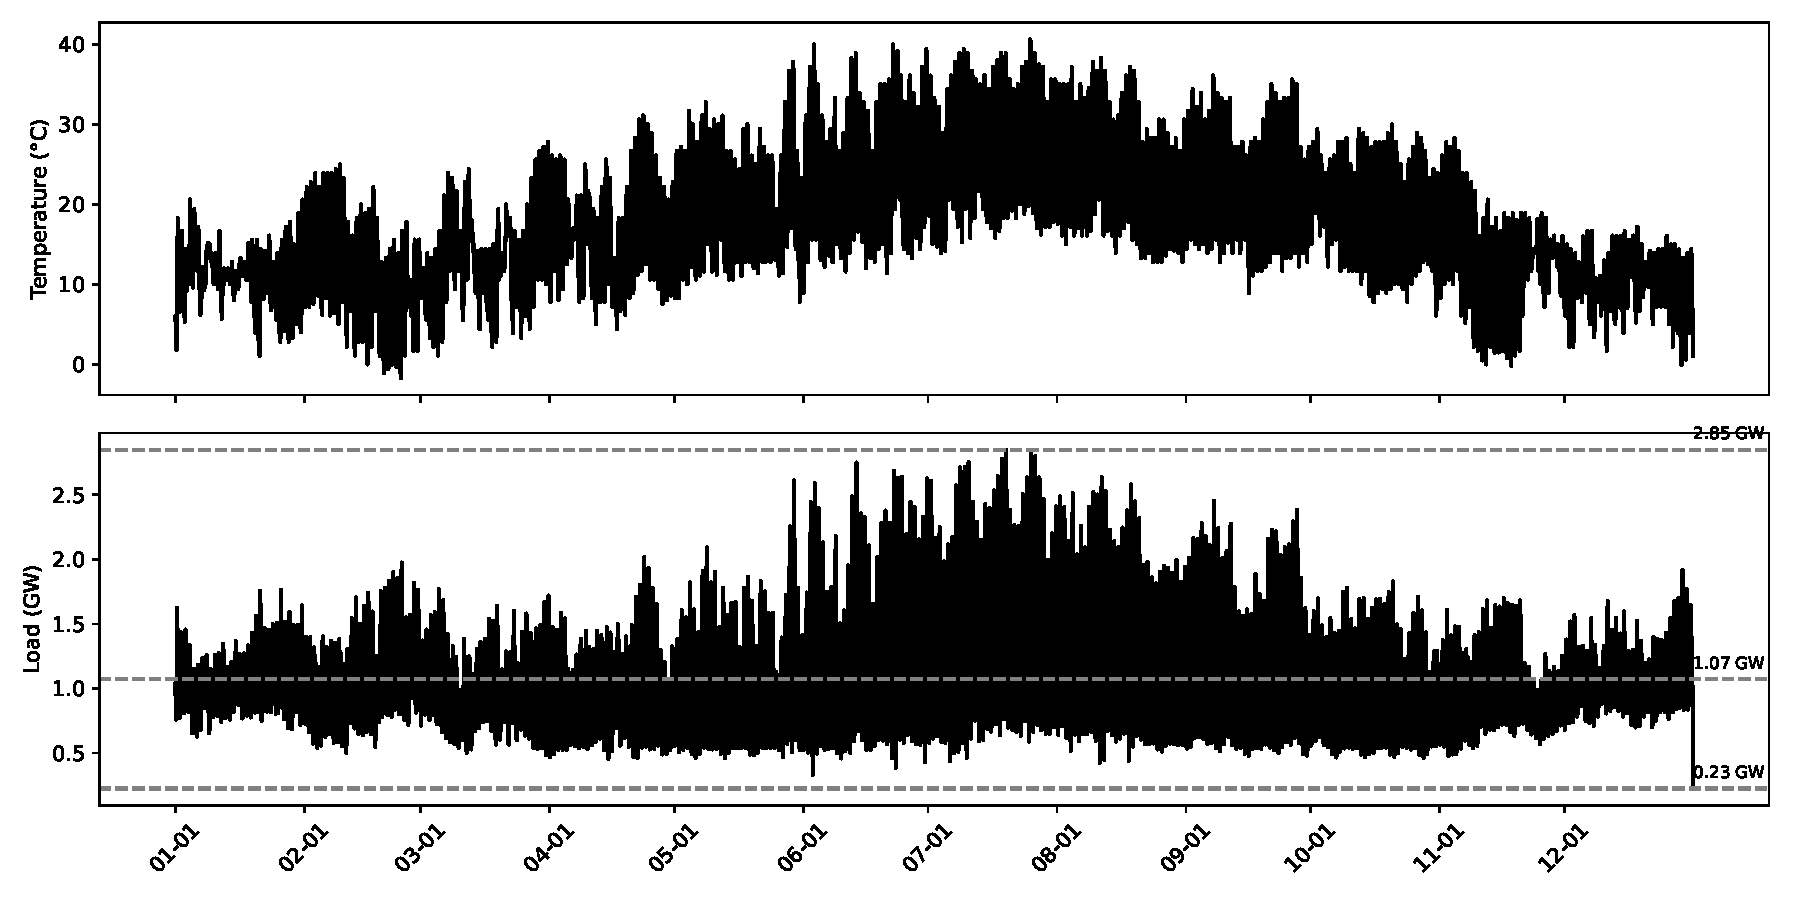
\includegraphics[width=0.8\columnwidth]{./figures/temp_load.pdf}
\end{figure}

\BIT
\item node in Central Valley part of WECC grid
\item year-long data sampled hourly
\item peak load and temperature in July
\EIT
	
\end{frame}

\begin{frame}{Preliminary analysis}
	
\begin{figure}
\centering
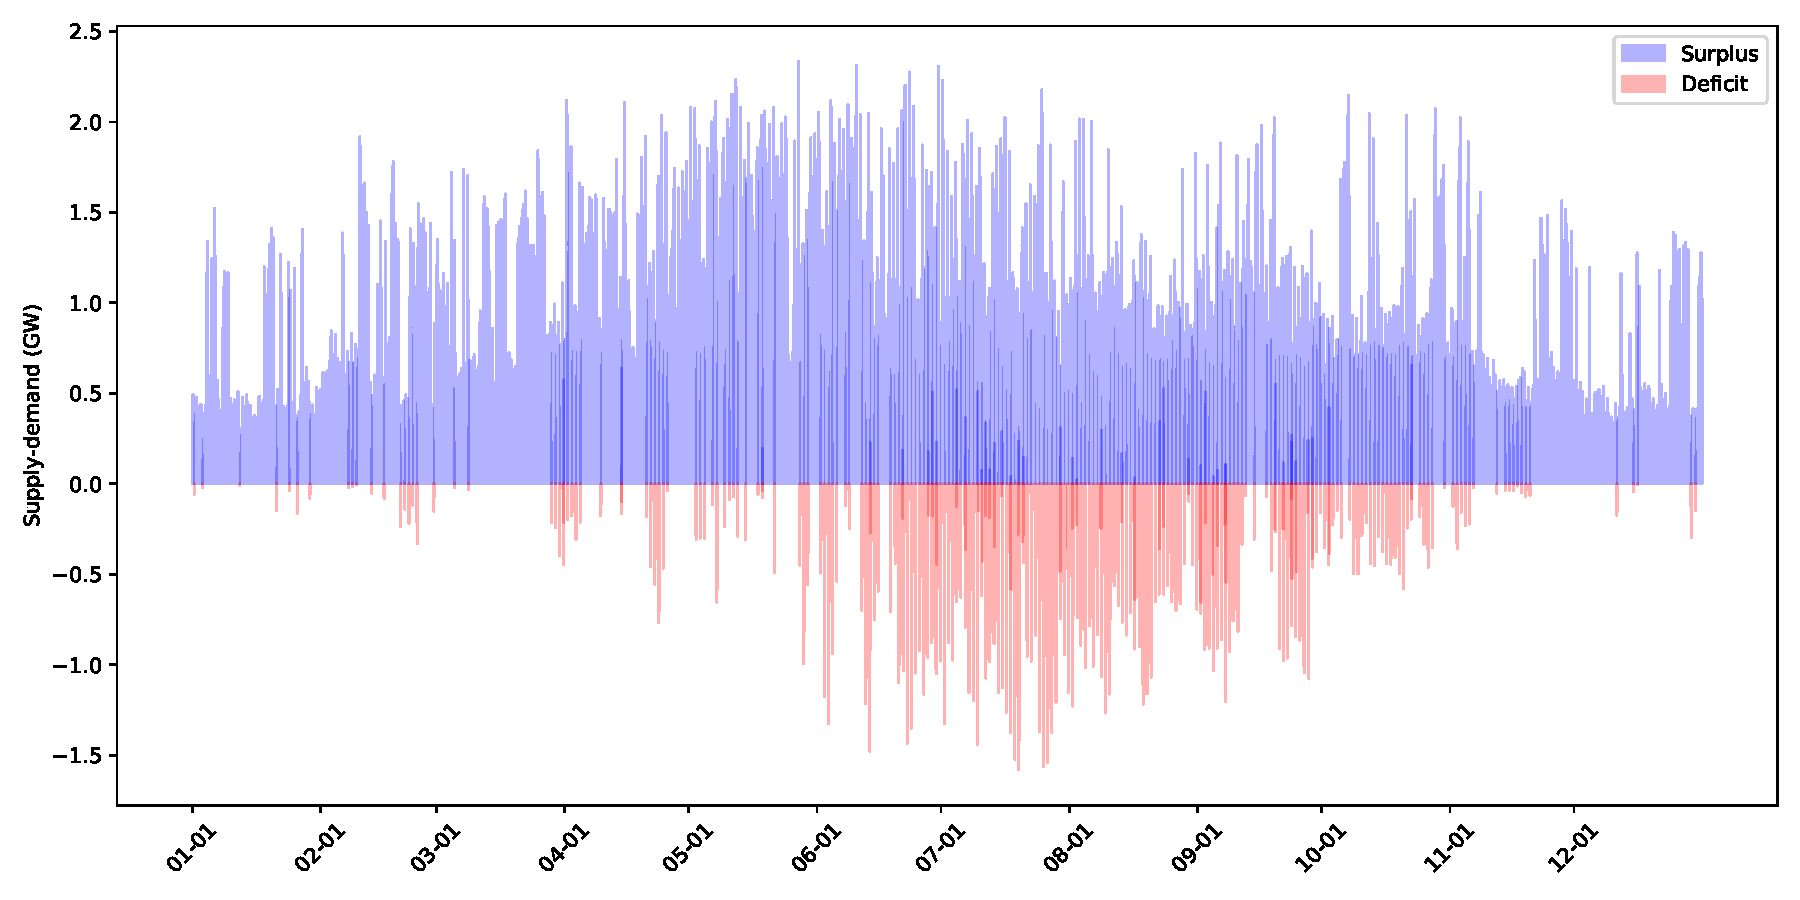
\includegraphics[width=0.8\columnwidth]{./figures/surplus_deficit.pdf}
\end{figure}

\BIT
\item total load is $\sum_{t=1}^{8760} l_t = 9404.96 \ \text{GWh}$
\item total possible generation is $\sum_{t=1}^{8760} (R_t + G) = 14232.15 \ \text{GWh}$ ($23\%$ renewable)
\item we can generate $4827.19 \ \text{GWh}$ more than we need
\item however we still have deficit in $10\%$ of the time 
\EIT
\end{frame}

\begin{frame}{Importance of storage}
    \BIT
    \item we have energy surplus, it just doesn't come at the right time
    \item we can reduce overall generation (fossil energy costs money)
    \item we need to `move' generation curve such that there are no deficits or surplus
    \item known as the optimal transport problem (measured by earth mover's distance)
    \item that is why a battery is indispensable
    \item analogy in finance: we have a portfolio of assets, we hold cash to rebalance risk
    \EIT
\end{frame}

\begin{frame}[fragile]{Prescient model \& implementation}
    \begin{columns}
        \begin{column}{0.46\textwidth}
    \[
        \begin{array}{ll}
            \mbox{minimize}   &  \frac{1}{T}\sum_{t=1}^{T} 10 s_t + 1.25 u_t + 0.5 u_t^2 \\
            \mbox{subject to} & q_1 = Q/2, \\
            & q_{T+1} = Q/2, \\
            & q_{t+1} = q_t - b_t, \; t = 1, \ldots, T, \\
            & b + r + u = l(1-s), \\
            & 0 \preceq s \preceq 1, \\
            & 0 \preceq r \preceq R, \\
            & 0 \preceq q \preceq Q \ones, \\
            & 0 \preceq u \preceq G \ones, \\
            & |b| \preceq B 1.
        \end{array}
    \]
    \vfill
    coefficients chosen arbitrarily to reflect 
    quadratic cost of fossil generation and high cost of 
    borrowing slack energy 
    \end{column}
    \begin{column}{0.54\textwidth}
\begin{lstlisting}[language=mypython, basicstyle=\footnotesize\ttfamily, belowskip=0em]
T = R.shape[0]
B = cp.Variable(nonneg=True)
b = cp.Variable(T)
q = cp.Variable(T+1, nonneg=True)
r = cp.Variable(T, nonneg=True)
u = cp.Variable(T, nonneg=True)
s = cp.Variable(T, nonneg=True)
cons = [
    q[0] == Q/2, q[-1] == Q/2, r <= R,
    q <= Q, u <= G, cp.abs(b) <= B,
    cp.diff(q) == -b, s <= 1,
    b + r + u == cp.multiply(l, 1-s)]
obj = 1/T*(10*cp.sum(s) + 1.25*cp.sum(u) 
        + 0.5*cp.sum_squares(u))
prob = cp.Problem(cp.Minimize(obj), cons)
\end{lstlisting}
    \vfill
    takes $\approx0.5$ seconds on average to compile and solve using Apple M2 CPU
    (remarkable considering the problem is not small: $T=8760$)
    \end{column}
    \end{columns}
\end{frame}

\begin{frame}{How much storage is enough?}
\begin{columns}
    \begin{column}{0.6\textwidth}
        \begin{figure}
            \centering
            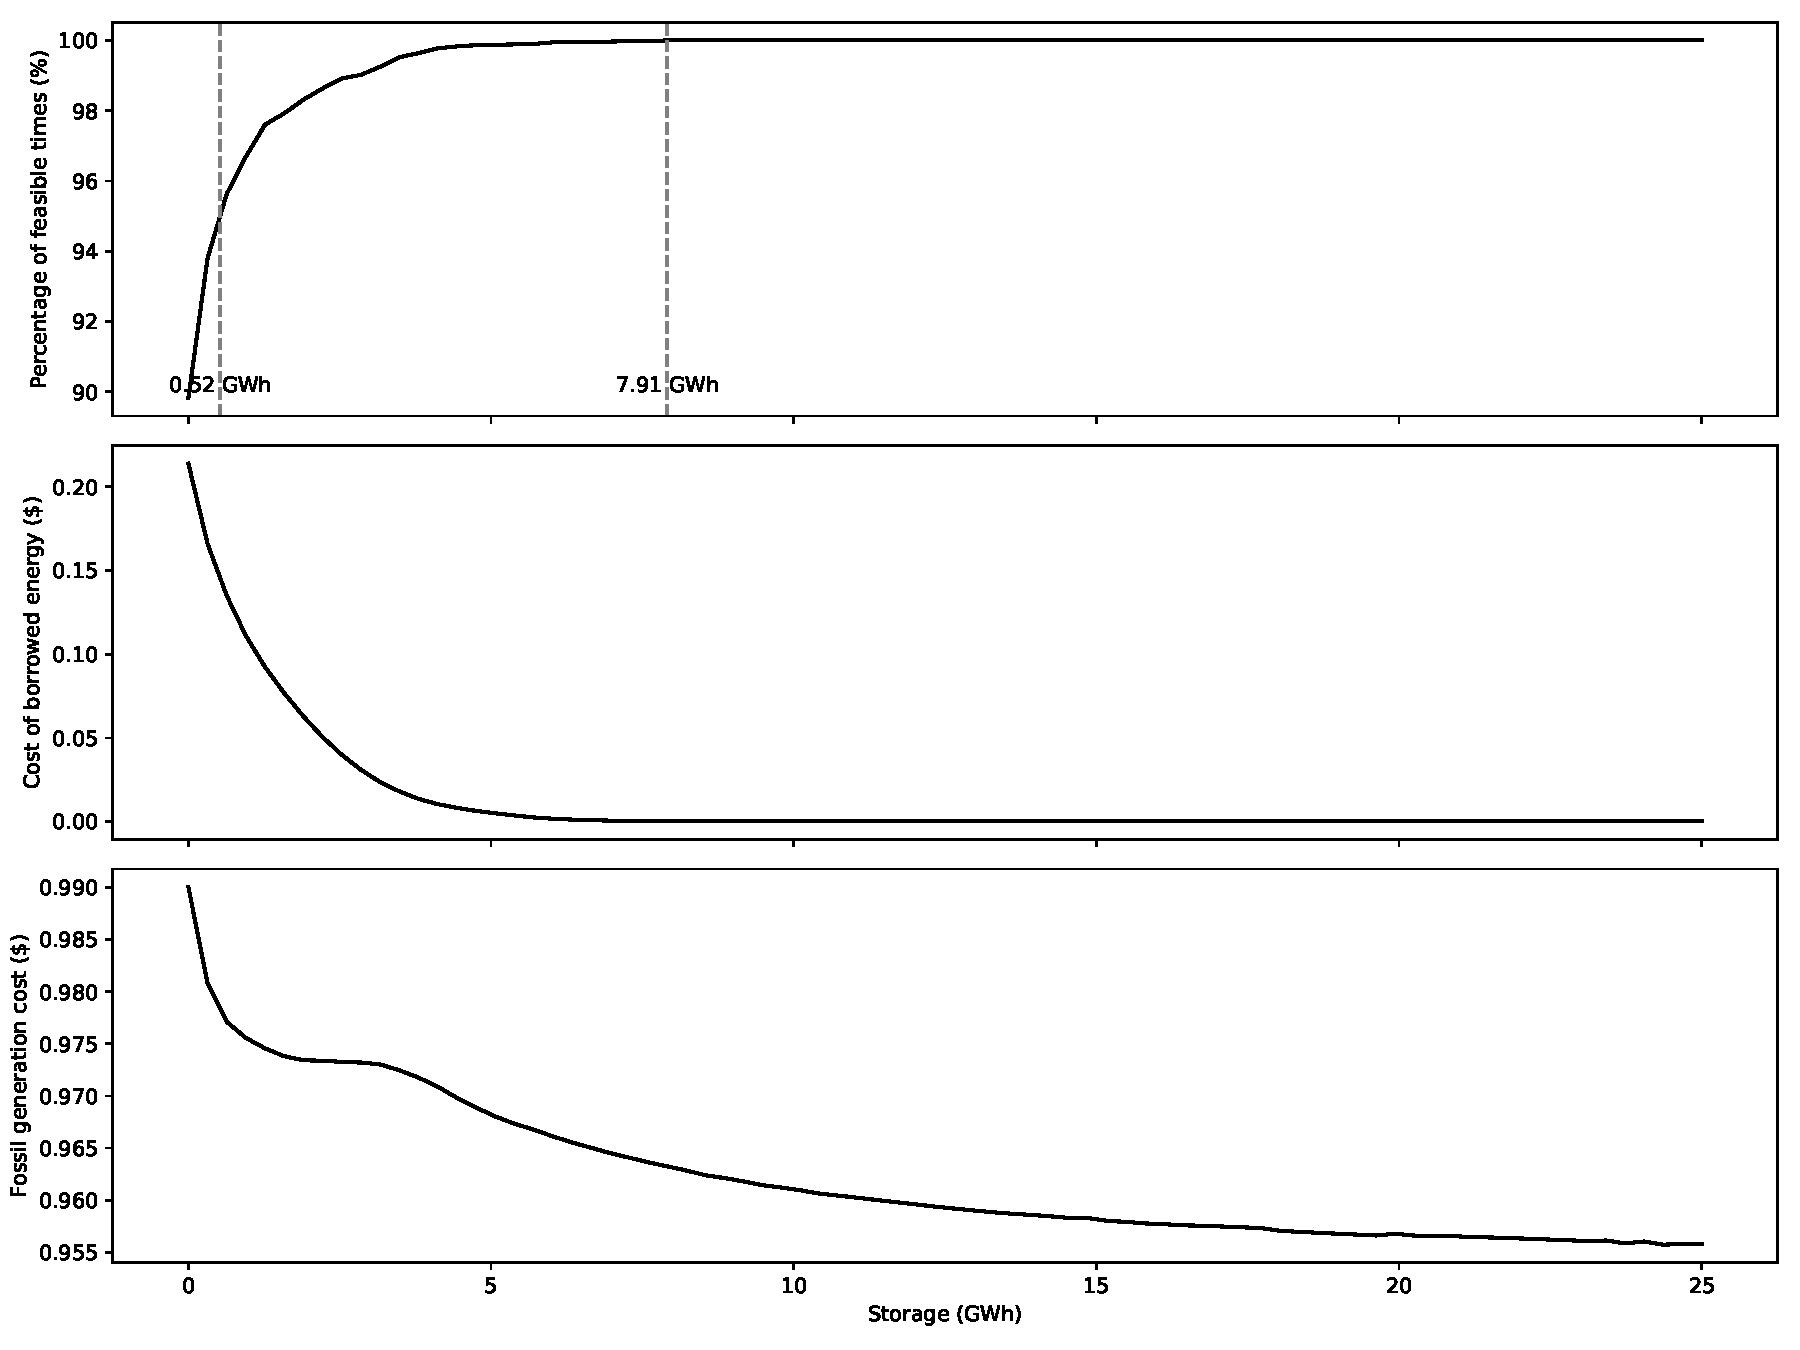
\includegraphics[width=\columnwidth]{./figures/storage_enough.pdf}
        \end{figure}
    \end{column}
    \begin{column}{0.4\textwidth}
        \begin{table}[ht]
            \centering
            \resizebox{\columnwidth}{!}{ % Scale the table to fit the column width
                \begin{tabular}{|c|c|c|}
                    \hline
                    \textbf{Storage (GWh)} & \textbf{Average fossil cost (\$)} & \textbf{Reliability (\%)} \\
                    \hline
                    0.01 & 0.99 & 90.05 \\
                    0.52 & 0.98 & 95.16 \\
                    2.79 & 0.97 & 98.98 \\
                    7.91 & 0.96 & 100.00 \\
                    25.00 & 0.96 & 100.00 \\
                    \hline
                \end{tabular}
            }
        \end{table}
        \begin{itemize}
            \item We require $7.91$ GWh of storage to eliminate all infeasible times ($\approx$ 1 week of load)
            \item $0.52$ GWh of storage is enough to reduce infeasible times by $50\%$ (just $6.5\%$ of required storage!)
        \end{itemize}
    \end{column}
\end{columns}
\end{frame}

\begin{frame}{Fossil generation profiles for different storage}
	
\begin{figure}
\centering
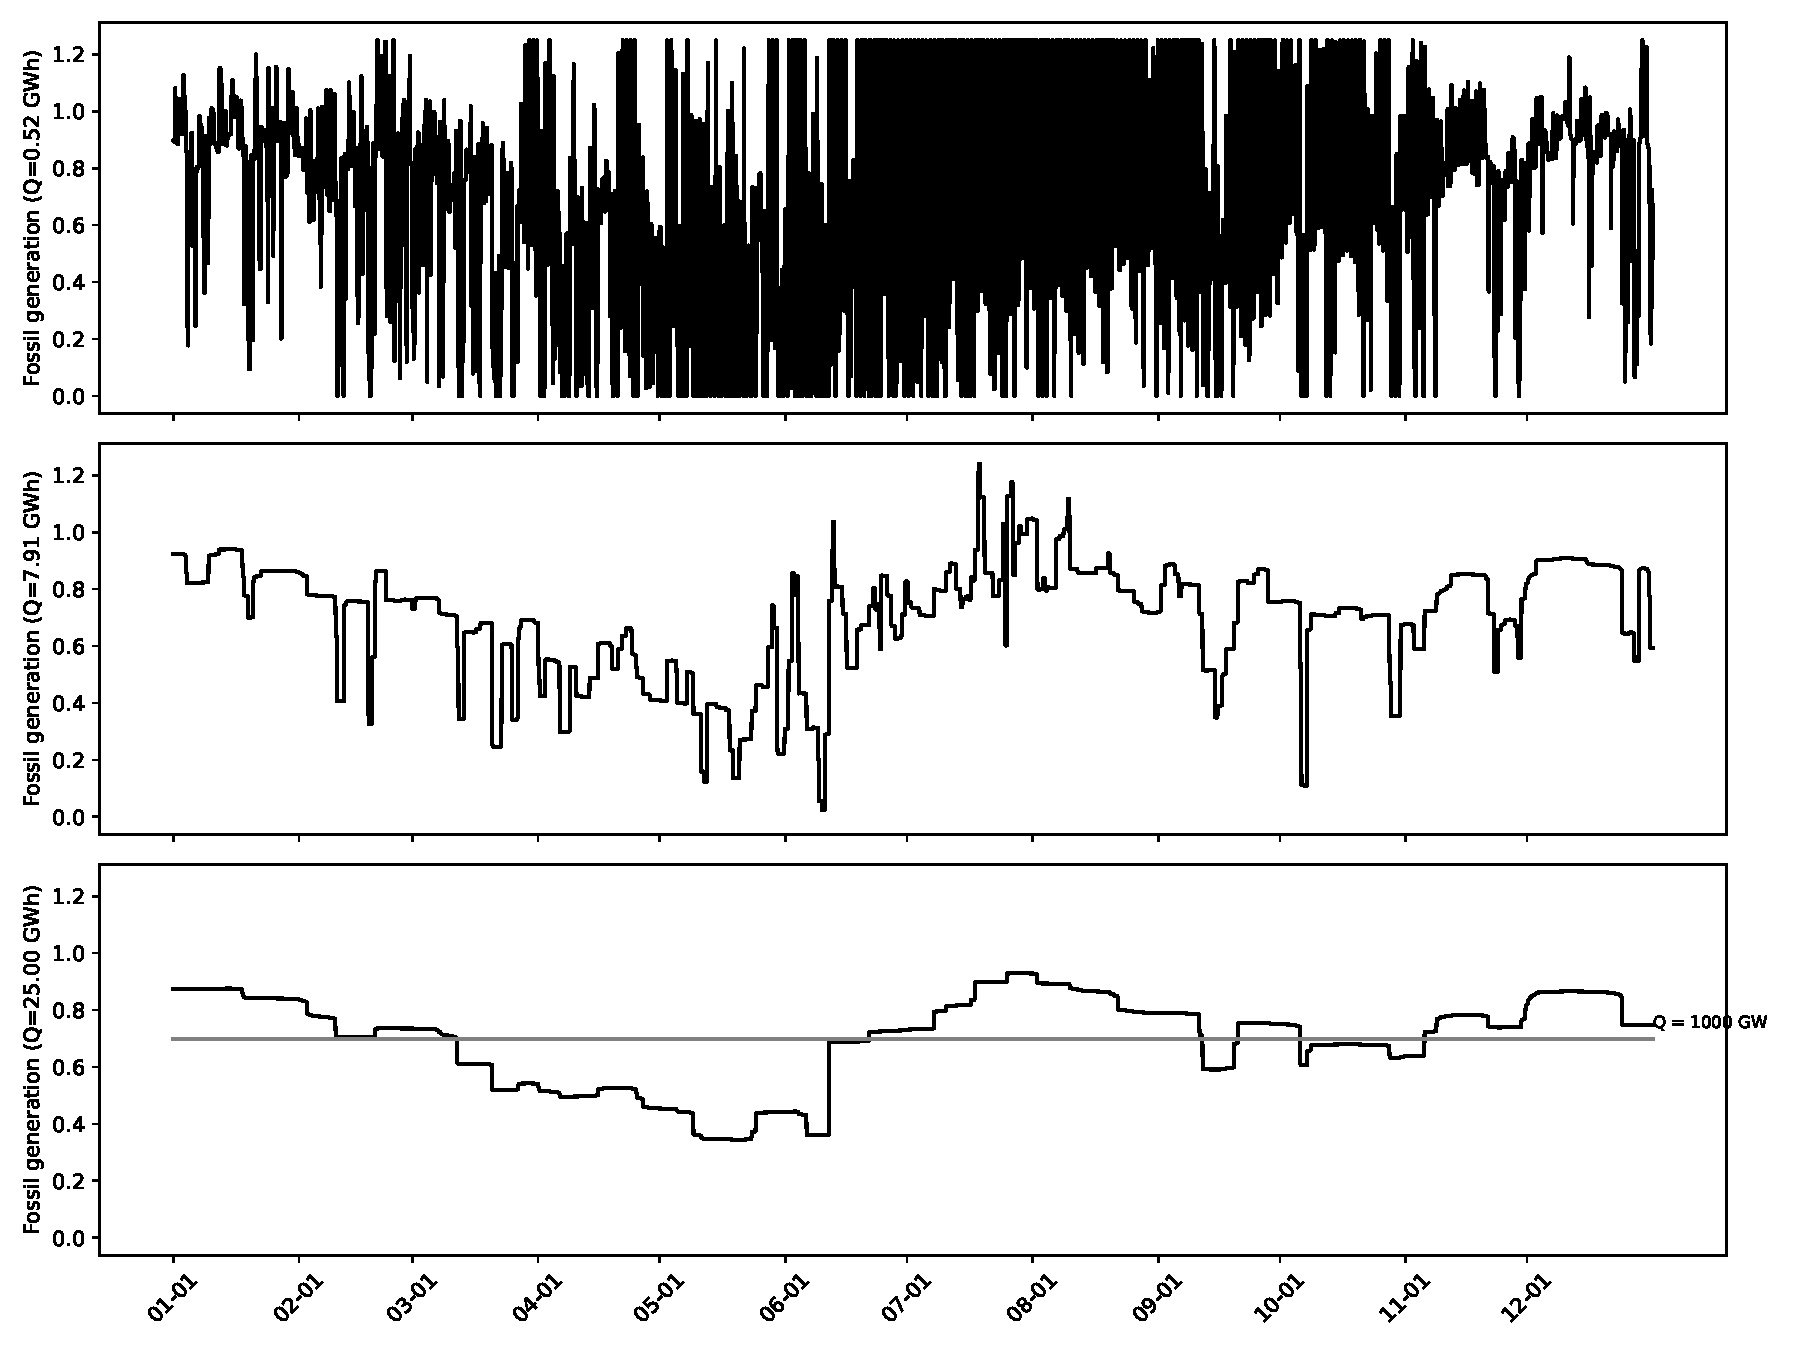
\includegraphics[width=0.5\columnwidth]{./figures/fossil_profiles.pdf}
\end{figure}

\BIT
\item fossil generation cost $\frac{1}{T}\sum_{t=1}^{T} 1.25 u_t + 0.5 u_t^2$ is strongly convex
\item if $u_t$ varies greatly, the quadratic term penalizes this variance heavily
\item by making $u_t$ more uniform (constant), we reduce the cost (\ie \ use Jensen's)
\item analogy in engineering: diesel engine's torque vs. RPM curve and why trucks have lots of wheels
\EIT
\end{frame}

\begin{frame}{Feasible case with minimum required storage}
\begin{columns}
    \begin{column}{0.6\textwidth}
        \begin{figure}
            \centering
            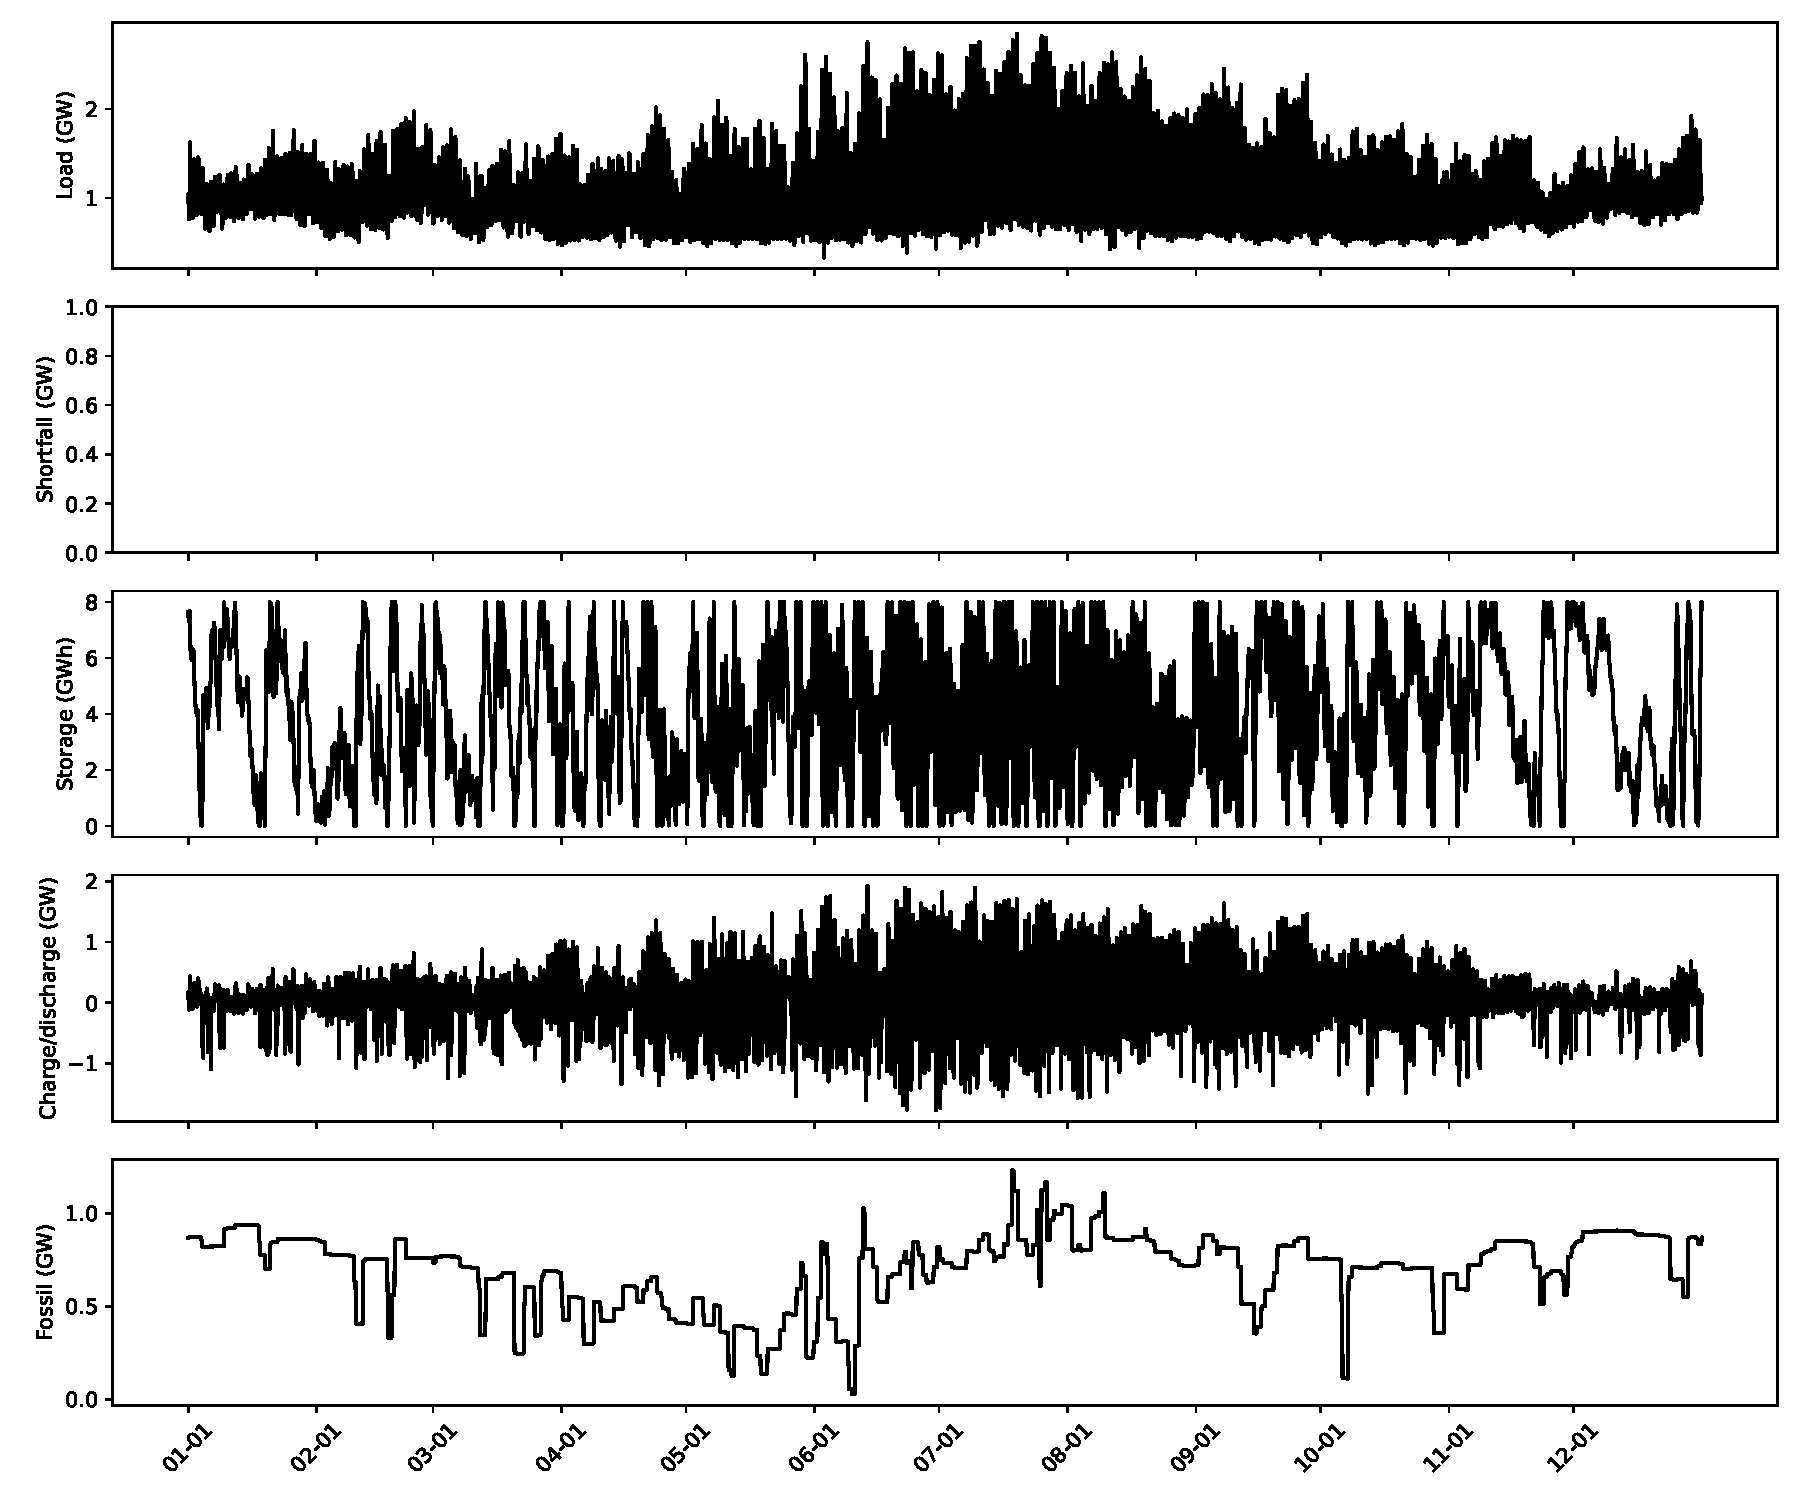
\includegraphics[width=\columnwidth]{./figures/hourly_profiles.pdf}
        \end{figure}
    \end{column}
    \begin{column}{0.4\textwidth}
        \begin{figure}
            \centering
            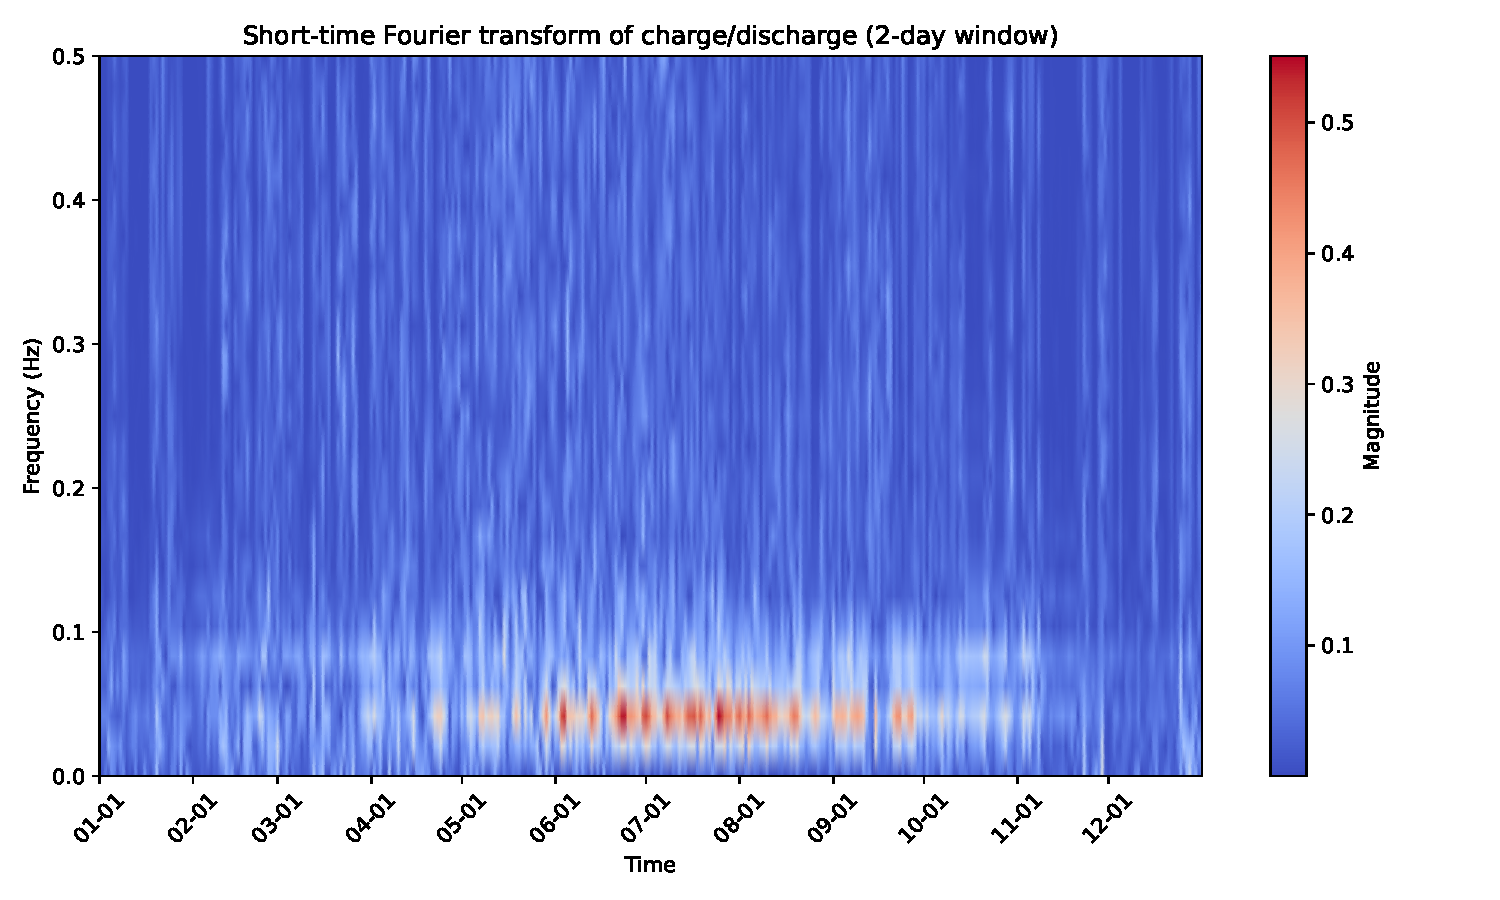
\includegraphics[width=\columnwidth]{./figures/stft_charge_2day_window.pdf}
        \end{figure}
            \BIT
            \item oscillations in charge/discharge increase in high-stress times (load peaks)
            \item same goes for oscillations in storage
            \item fossil generation approaches its maximum in these times
            \EIT
        \end{column}
\end{columns}
\end{frame}

\begin{frame}{Final remarks} 
\BIT
\item \textbf{in this prescient single-node model, we:}  \\
\hspace{12mm} $-$ showed the importance of storage in reducing fossil generation costs\\
\hspace{12mm} $-$ showed that the fossil generation profile is smoother with more storage\\
\hspace{12mm} $-$ analyzed minimum required storage for feasibility\\
\hspace{12mm} $-$ analyzed storage, charging and energy generation profiles\\
\item \textbf{next steps:} \\
\hspace{12mm} $-$ refine our reliability analysis\\
\hspace{12mm} $-$ current formulation allows for charging with borrowed energy\\
\hspace{12mm} $-$ but preventing this results in non-convex problem\\
\hspace{12mm} $-$ develop convex heuristics for a more detailed reliability analysis\\
\hspace{12mm} $-$ move on from prescient case to MPC using forecasts\\
\EIT
\end{frame}
    

\begin{frame}{Outreach \& dissemination}
\begin{columns}
    \begin{column}{0.6\textwidth}
        \begin{figure}
            \centering
            
\includegraphics[width=\columnwidth]{./figures/cybercon_program.png}
        \end{figure}
    \end{column}
    \begin{column}{0.4\textwidth}
        \begin{itemize}
            \item participated in 2024 Cybersecurity \& Technology Innovation Conference
            \href{https://www.doecybercon.com/Program/Agenda}{(click to acces the program \& slides)}
            \item abstract accepted to 2024 EU PVPMC
            \href{https://www.sandia.gov/app/uploads/sites/243/dlm_uploads/2024/08/2024-European-PVPMC-Program-V9.pdf}{(click to acces the program)}
            \item currently working on a manuscript
        \end{itemize}
    \end{column}
\end{columns}
\end{frame}
    


	

\end{document}
